\chapter{Experimental setup and methodology}
\label{ch4:anchor:chapter}

\section{Introduction}
In this chapter, the aim of the experiment, the experimental procedure, the materials, the analyses of samples, and the detailed experimental methods employed are all concisely described. Analyses of the methods and testing standards used are provided. All the parameters used are discussed and shown, and the safety precautions are followed throughout the experiments. After the \acrshort{afff} concentrate has been reacted with various engineering materials, the functional groups, particle shape and size, particle size distribution, and elemental composition are critically analyzed.

\section{Aim of the experiment}
The experimental work aims to evaluate and assess the impact and compatibility of the materials used to construct the storage facility with the \acrshort{afff} concentrate. The incompatibility of these materials can greatly influence the performance parameters of an \acrshort{afff} solution.  

\section{Methodology}
Samples of stainless steel, mild steel, and \acrshort{hdpe}, together with \acrshort{afff} concentrate, were carefully prepared. A guillotine machine was used to cut the material sheets into the desired shapes and sizes. All the material sheets were cut to the same sizes and shapes for a fair comparison. A total of three samples were used during the experiments. These sample materials were exposed to natural environmental conditions for 3 months. All the samples were then immersed and soaked in a 3\% proportion of \acrshort{afff} concentrate for 5 months. \Acrfull{ftir}, \acrfull{tem}, \acrfull{dls}, and \acrfull{icp} wet analysis were performed on samples of \acrshort{afff} concentrate. This was done to analyze any critical changes in the parameters of \acrshort{afff} concentrate after being in reaction with these materials. All the findings were carefully recorded and analyzed. However, it should be noted that the objective was to analyze the \acrshort{afff} concentrate, not the engineering materials. The experimental procedure followed for all the samples is presented in the flowchart in Figure \ref{ch4:figure:procedure}. 

\begin{figure}[H]
\centering

\begin{tikzpicture}[node distance=3.8cm]
    \tikzstyle{block} = [rectangle, minimum height=1.5cm, inner sep=1em, text centered, text width=5cm, draw=black]
    \tikzstyle{arrow} = [thick, ->, >=stealth]

    \node (prepare) [block] {Prepared materials and \acrshort{afff} concentrate samples};

    \node (expose) [block, below of=prepare] {Exposed material samples to natural environmental conditions 3 months};

    \node (immerse) [block, below of=expose] {Immersed and soaked material samples to \acrshort{afff} solution for 5 months};

    \node (use) [block, right of=prepare, xshift=6cm] {Used \acrshort{ftir}, \acrshort{tem}, \acrshort{dls} and \acrshort{icp} intruments to test the \acrshort{afff} concentrate};

    \node (analyse) [block, below of=use] {Analysed the functional groups, particle sizes and shapes, particle size distribution, and elemental composition of the \acrshort{afff} concentrate};

    \node (record) [block, below of=analyse] {Data recording};

    \newcommand*{\connector}[4][]{
        \draw[#1] (#3) -| ($(#3) !#2! (#4)$) |- (#4);
    }

    \draw [arrow] (prepare) -- (expose);
    \draw [arrow] (expose) -- (immerse);

    \connector[->, black]{0.5}{immerse}{use}

    \draw [arrow] (use) -- (analyse);
    \draw [arrow] (analyse) -- (record);

\end{tikzpicture}

\caption{Typical experimental procedure}
\label{ch4:figure:procedure}
\end{figure}

\section{Sample preparation}
\subsection{Material plates}
The 3, 4, and 5 mm thick sheets of mild steel, The 3, 4, and 5 mm thick sheets of mild steel, stainless steel, and \acrshort{hdpe}, respectively, were prepared for the experiments. The stainless steel was provided specially by Columbus Stainless (Pty) Ltd. The sizes are based on the common thickness of the storage tanks that contain the \acrshort{afff} concentrate, as investigated by \cite{protopopoff2011surface}.

These sheets were required to be cut to the desired shapes and sizes so that they could fit in 800 ml beakers filled with \acrshort{afff} concentrate. The scriber was used to scribe the precise sizes and shapes to be cut. This was done at the Durban University of Technology (DUT) manufacturing workshop using a guillotine-cutting machine. The prepared material samples can be seen in Figure \ref{ch4:figure:samples} (a-c).

\begin{figure}[H]
    \centering
    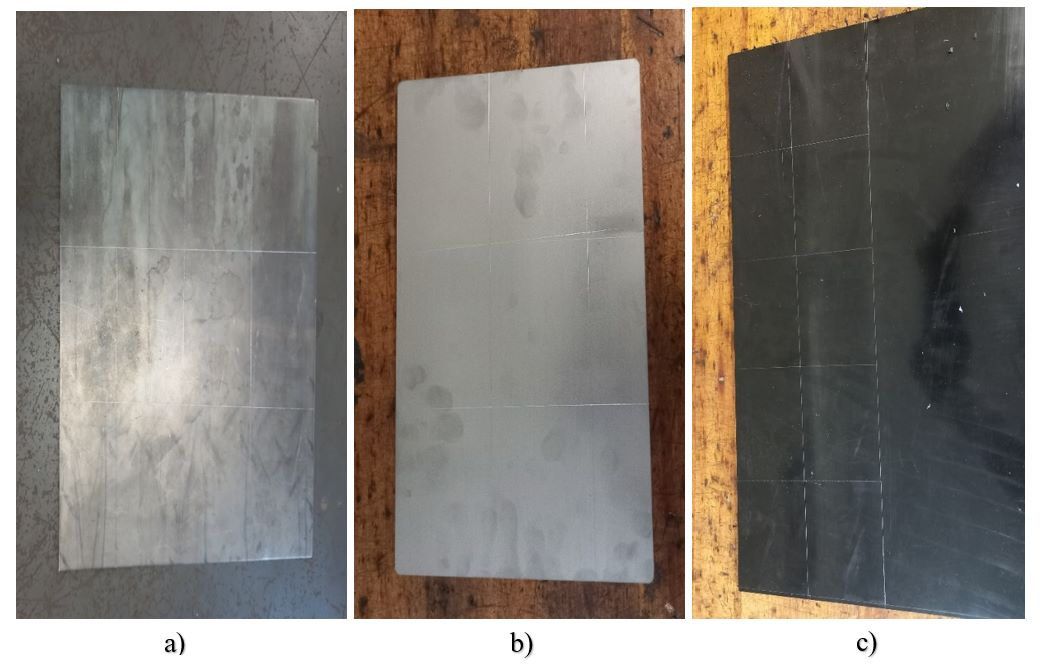
\includegraphics[width=\textwidth]{new_fig_3.jpg}
    \caption{Mild steel (a), stainless steel (b), and HDPE (c).}
    \label{ch4:figure:samples}
\end{figure}

\subsection{The cutting process}
The prepared samples were cut to sizes 60 mm by 100 mm using a guillotine machine. It can be seen in Figure \ref{ch4:figure:samples} (a-c) that the samples were first scribed before being cut to ensure precision. Mild steel and stainless steel were cut using a guillotine that can cut up to a thickness of 5 mm. In contrast, \acrshort{hdpe} was cut with a guillotine that can cut up to 3 mm of thickness, as it is not as hard as the two sheets of steel. Figure \ref{ch4:figure:guillotines} (a-b) shows the two guillotine machines that were used to cut the samples.

\begin{figure}[H]
    \centering
    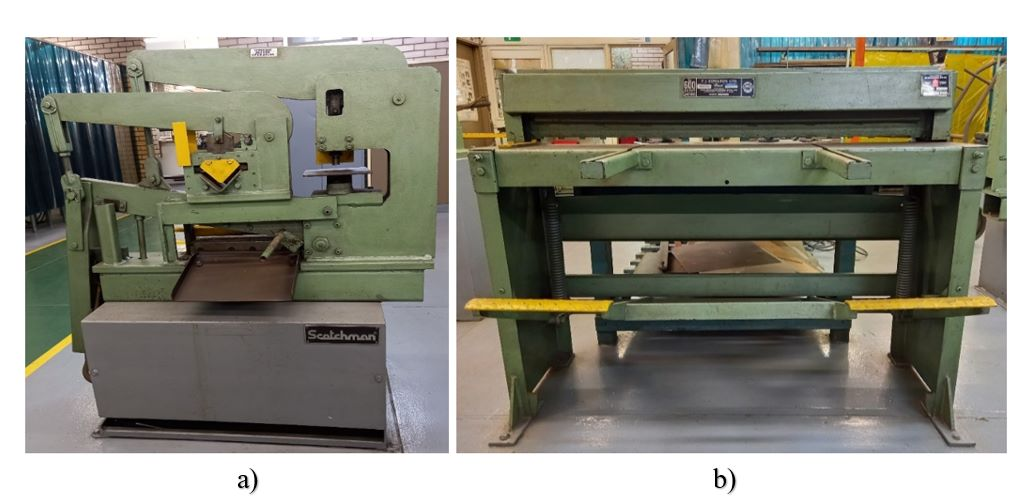
\includegraphics[width=\textwidth]{3mm_and_5mm_guillotine_machine.jpg}
    \caption{Guillotine machines that cuts up to 5 (a) and 3mm (b) thickness, respectively.}
    \label{ch4:figure:guillotines}
\end{figure}

As aforementioned, the samples were cut into numerous pieces in the desired shapes and sizes to fit in the 800 ml glass beakers. Figure \ref{ch4:figure:samples_cut} shows the samples after the cutting process.

\begin{figure}[H]
    \centering
    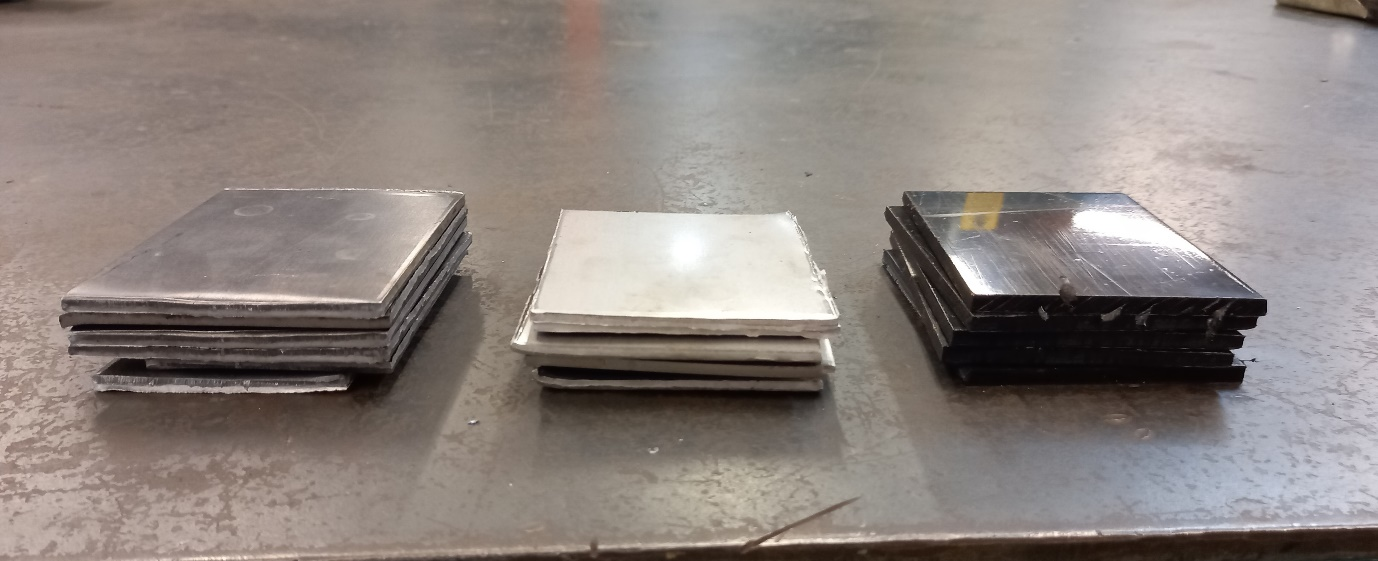
\includegraphics[width=\textwidth]{samples_after_being_cut.jpg}
    \caption{Samples after being cut to the desired sizes, mild steel, stainless steel, and HDPE (left to right).}
    \label{ch4:figure:samples_cut}
\end{figure}

The samples were polished and cleaned using the rectangular file. This was done to remove the roughness and dangerous chips, to avoid any possible injuries during the experimental setup. Figure \ref{ch4:figure:file_and_vice} shows the tools used when cleaning and polishing the samples.
 
\begin{figure}[H]
    \centering
    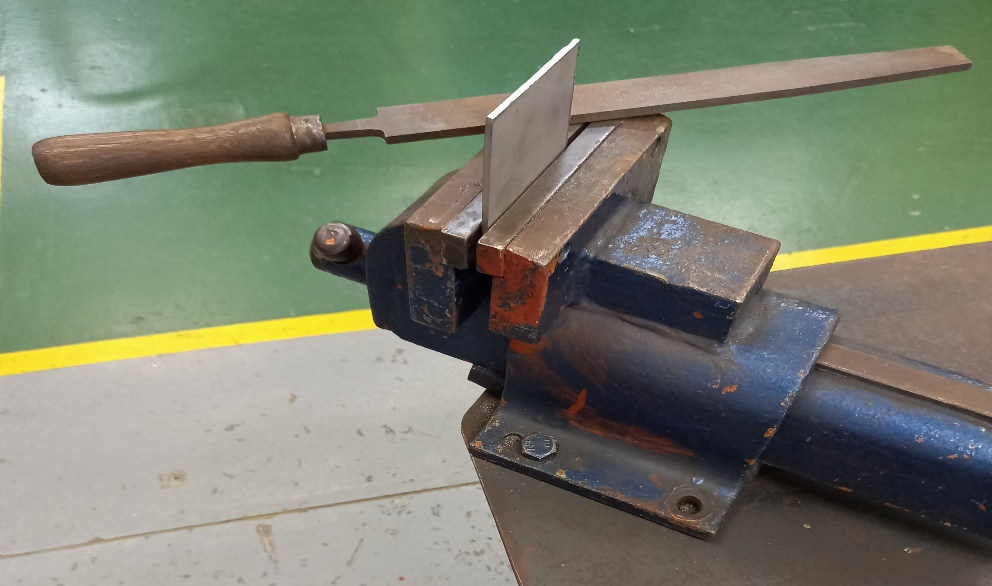
\includegraphics[width=.6\textwidth]{rectangular_file_and_bench_vice.jpg}
    \caption{Rectangular file and bench vice}
    \label{ch4:figure:file_and_vice}
\end{figure}

\subsection{AFFF concentrate samples}
The 3\% \acrshort{afff} concentrate samples were prepared in 20-liter batches and kept at room temperature in the DUT laboratory. These were carefully stored in their original containers until the material sheet samples were available and ready. Figure \ref{ch4:figure:suplier} shows the \acrshort{afff} concentrate from the supplier in its original 20-liter container.
 
\begin{figure}[H]
    \centering
    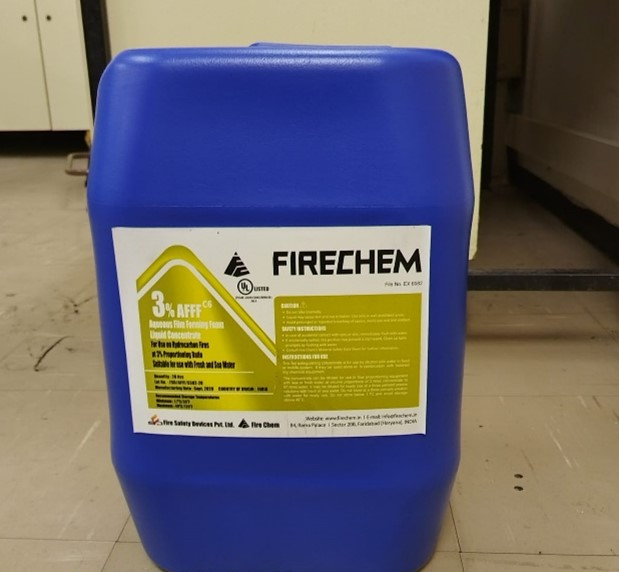
\includegraphics[width=.5\textwidth]{pure_afff_concentrate_from_supplier.jpg}
    \caption{Pure \acrshort{afff} concentrate from the supplier.}
    \label{ch4:figure:suplier}
\end{figure}

To immerse various material samples, \acrshort{afff} concentrate was filled in respective glass beakers. Figure \ref{ch4:figure:immersed} shows the three glass beakers used to immerse the three materials of interest.
 
\begin{figure}[H]
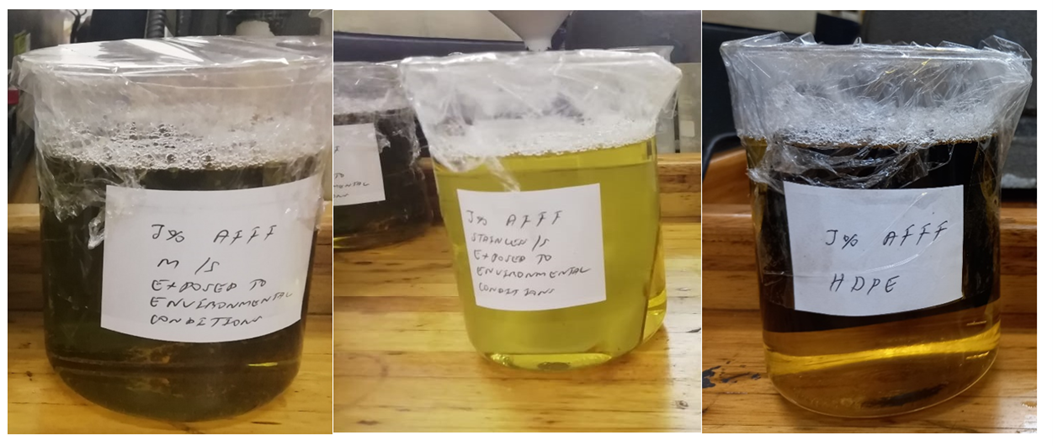
\includegraphics{mild_stainless_steel_and_hdpe_immersed_in_afff_concentrate.png}
\caption{Mild steel, stainless steel, and HDPE (left to right) samples immersed in AFFF}
\label{ch4:figure:immersed}
\end{figure}

\subsection{Experimental matrix}

\begin{table}[H]
\centering
\caption{Experimental matrix with \acrshort{afff} concentrate.}

\renewcommand{\arraystretch}{2.5}
\begin{tabularx}{\textwidth}{ XXX }
    \hline
    Material & Instrument & Analyses \\
    \hline
    \acrshort{afff} concentrate & \acrshort{ftir} & Functional groups \\
    & \acrshort{tem} & Particle size and shape \\
    & & HR imaging \\
    & & Electron diffraction images \\
    & \acrshort{dls} & Particle size \\
    & & Particle size distribution \\
    & \acrshort{icp} & Elementary identification \\
    \hline
\end{tabularx}

\end{table}

\section{Testing} 
The different tests that were performed after the experiments are discussed in this section. The apparatus and various materials used to conduct the tests are concisely described.

\subsection{Fourier transform infrared spectroscopy (FTIR)}
All the \acrshort{afff} concentrate samples were analyzed using the \acrshort{ftir} technique. This was accomplished by comparing the manufacturer's pure \acrshort{afff} concentration to others that had reacted with the materials of interest. The \acrshort{ftir} analysis assisted in identifying the functional groups for various exposed samples, and the instrument can be seen in Figure \ref{ch4:figure:ftir}.
 
\begin{figure}[H]
    \centering
    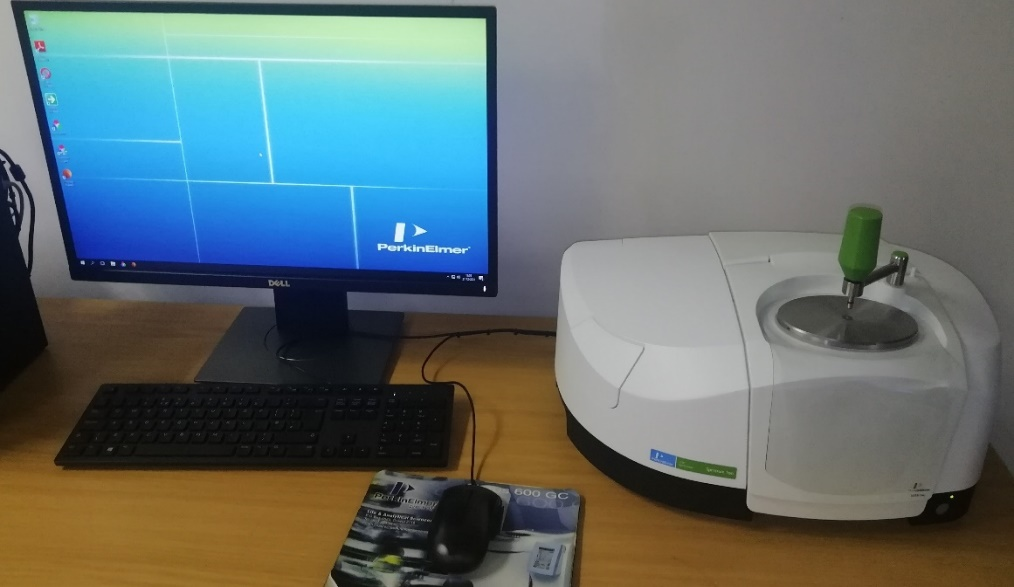
\includegraphics[width=.75\textwidth]{ftir_instrument.jpg}
    \caption{FTIR instrument used to identify the functional groups.}
    \label{ch4:figure:ftir}
\end{figure}

\subsection{Transmission electron microscopy (TEM)}
Since the \acrshort{ftir} does not provide conclusive information, it was essential to validate the \acrshort{ftir} analysis with other tests. \acrshort{tem} analyses were conducted to analyze the overall particle shape and the visual overall size of the \acrshort{afff} concentrate particles using HR imaging and electron diffraction images. It should be noted that \acrshort{tem} does not provide sufficient information on how the particles in the exposed \acrshort{afff} concentrate are distributed and does not convey precise particle sizes. Consequently, the other relevant tests were necessary. The \acrshort{tem} instrument used for the tests is depicted in Figure \ref{ch4:figure:tem}.
 
\begin{figure}[H]
    \centering
    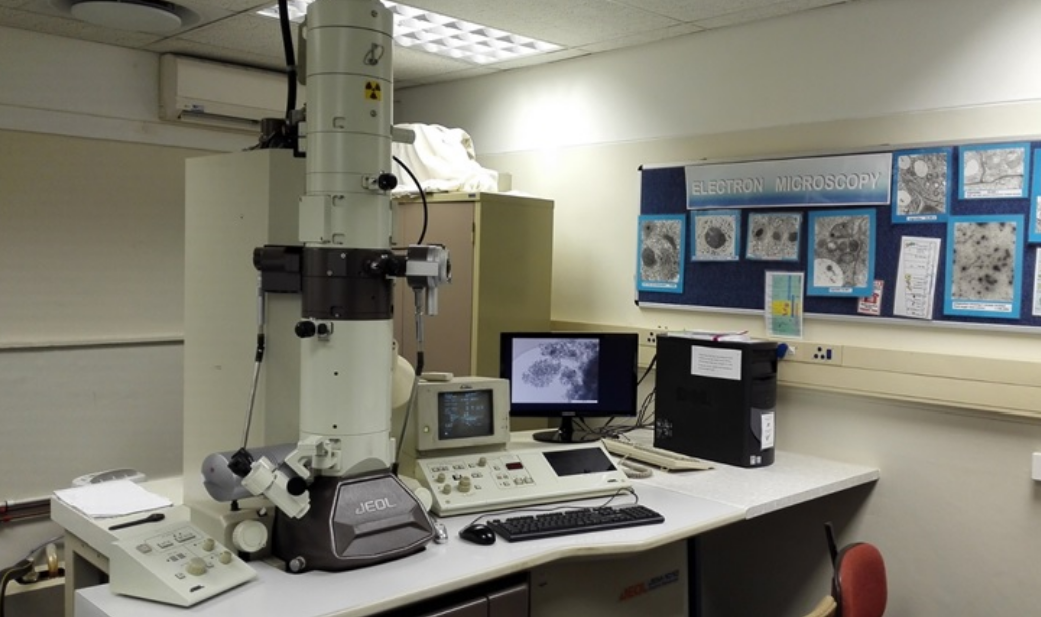
\includegraphics[width=.75\textwidth]{tem_instrument.png}
    \caption{TEM instrument used to analyze AFFF concentrate particles.}
    \label{ch4:figure:tem}
\end{figure}

\subsection{Dynamic Light Scattering (DLS)}
The \acrshort{dls} tests were conducted to deduce the particle size distribution and precise particle sizes using the instruments shown in Figure \ref{ch4:figure:dls}. This was achieved by measuring the hydrodynamic diameter (Z-average) of any present particles in units of nm. This was done to validate the findings of \acrshort{tem}, and it furthered an in-depth understanding of the behaviour of the \acrshort{afff} concentrate particles when exposed to various materials and how these materials affect their performance parameters.
 
\begin{figure}[H]
    \centering
    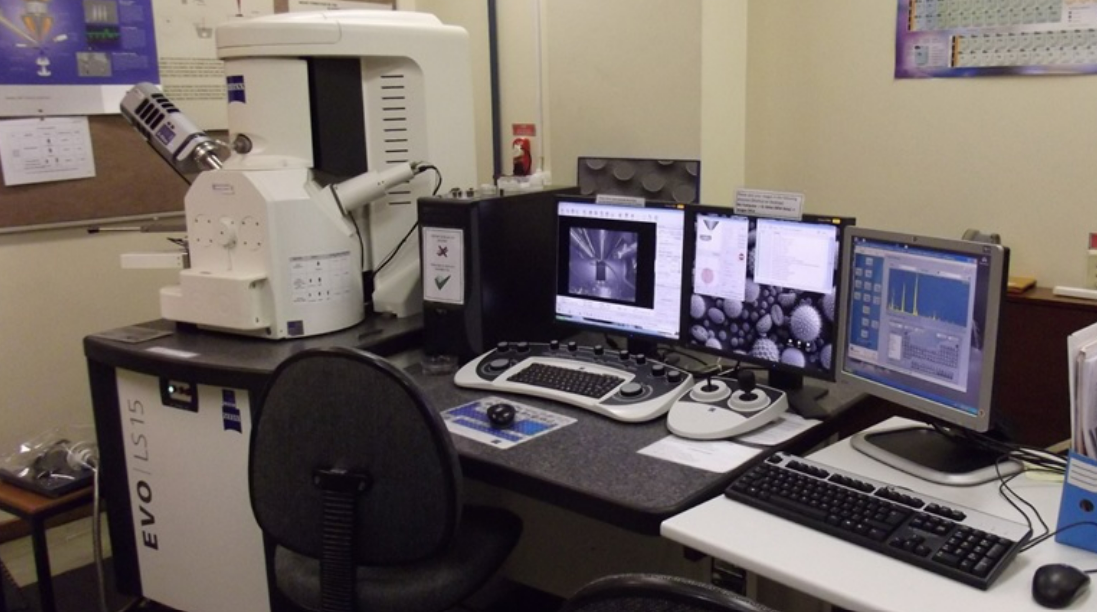
\includegraphics[width=.75\textwidth]{dls_instrument.png}
    \caption{DLS instrument used to analyze particle distribution of AFFF concentrate.}
    \label{ch4:figure:dls}
\end{figure}

\subsection{Inductively Coupled Plasma Atomic Emission Spectroscopy (ICP-AES)}
Finally, \acrshort{icp-aes} tests were performed to determine the elemental composition of the exposed \acrshort{afff} concentrate and compare it to the standard qualities. The changes in elemental composition can greatly affect the properties, hence the performance of \acrshort{afff} during firefighting circumstances. Thus, it is vital to assess the impact of the various materials on the composition of the \acrshort{afff} concentrate. Figure \ref{ch4:figure:icp-aes} shows the \acrshort{icp-aes} instrument used during the tests.
 
\begin{figure}[H]
    \centering
    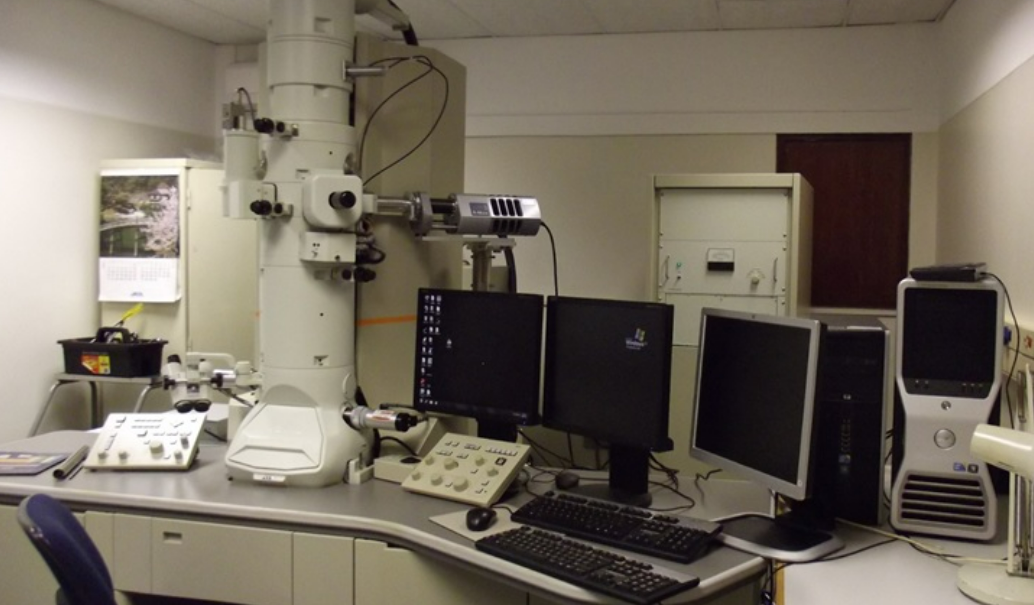
\includegraphics[width=.75\textwidth]{icp_instrument.png}
    \caption{ICP-AES instrument used for elementary analysis.}
    \label{ch4:figure:icp-aes}
\end{figure}

\section{Conclusion}
The present chapter outlined the aim of the experiment, the material description, sample preparation, the techniques employed to test the samples and as well as the equipment and testing standards used. The instruments used for analyzing the \acrshort{afff} concentrate samples were presented with a thorough explanation of the purpose of each test. The experimental procedure followed in this investigation was explained. The results of the investigation are presented in Chapter \ref{ch5:anchor:chapter}.